\documentclass[tikz,border=10pt]{standalone}
\usetikzlibrary{calc}
\begin{document}
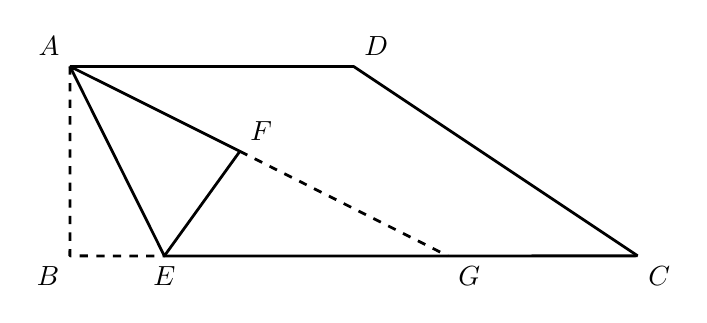
\begin{tikzpicture}[line width=1.0pt, line join=round]
\coordinate (A) at (-3.611,1.210);
\coordinate (B) at (-3.612,-1.196);
\coordinate (C) at (3.599,-1.196);
\coordinate (D) at (-0.006,1.208);
\coordinate (F) at (-1.453,0.132);




\coordinate (E) at (-2.412,-1.197);   
\coordinate (G) at (1.187,-1.196);    


\draw (A) -- (D) -- (C);              
\draw (E) -- (C);                     
\draw (A) -- (E) -- (F) -- (A);       


\draw[dashed] (A) -- (B) -- (E);      
\draw[dashed] (F) -- (G);             


\node[above left,  font=\fontsize{10}{12}\selectfont] at (A) {$A$};
\node[below left,  font=\fontsize{10}{12}\selectfont] at (B) {$B$};
\node[below right, font=\fontsize{10}{12}\selectfont] at (C) {$C$};
\node[above right, font=\fontsize{10}{12}\selectfont] at (D) {$D$};
\node[below,       font=\fontsize{10}{12}\selectfont] at (E) {$E$};
\node[above right, font=\fontsize{10}{12}\selectfont] at (F) {$F$};
\node[below right, font=\fontsize{10}{12}\selectfont] at (G) {$G$};
\end{tikzpicture}
\end{document}